% =========================
% L21.tex
% =========================

\chapter{L21 -- Funzioni definite in segno e teorema diretto di Lyapunov}
\label{chap:L21}

\section{Richiamo: funzioni definite in segno}

In questa lezione introduciamo uno degli strumenti più importanti per lo studio della stabilità dei sistemi non lineari: il \emph{metodo diretto di Lyapunov}.  
Prima, però, serve chiarire il significato di \emph{funzione definita in segno}.

Sia
\[
V:\mathbb{R}^n \to \mathbb{R},
\]
continua in un intorno dell'origine. Indichiamo con
\[
B_r=\{x\in\mathbb{R}^n:\|x\|<r\}
\]
la palla aperta di raggio \(r\) centrata nell'origine, e con
\[
\overline{B}_r=\{x\in\mathbb{R}^n:\|x\|\le r\}
\]
la corrispondente palla chiusa.

\subsection{Definizioni}

Diremo che \(V\) è:

\begin{itemize}
    \item \textbf{positiva definita} in \(B_r\) se
    \[
    V(0)=0,
    \qquad
    V(x)>0 \quad \forall x\in B_r\setminus\{0\};
    \]

    \item \textbf{positiva semidefinita} in \(B_r\) se
    \[
    V(0)=0,
    \qquad
    V(x)\ge 0 \quad \forall x\in B_r;
    \]

    \item \textbf{negativa definita} in \(B_r\) se \(-V\) è positiva definita, cioè
    \[
    V(0)=0,
    \qquad
    V(x)<0 \quad \forall x\in B_r\setminus\{0\};
    \]

    \item \textbf{negativa semidefinita} in \(B_r\) se \(-V\) è positiva semidefinita, cioè
    \[
    V(0)=0,
    \qquad
    V(x)\le 0 \quad \forall x\in B_r.
    \]
\end{itemize}

Se una funzione assume sia valori positivi sia valori negativi arbitrariamente vicini all'origine, allora si dice \textbf{indefinita} o \textbf{non definita in segno}.

\medskip

\noindent
L'idea intuitiva è semplice:
\begin{itemize}
    \item una funzione positiva definita ``misura una distanza energetica'' dall'origine;
    \item una funzione negativa definita è il suo opposto;
    \item una funzione semidefinita può annullarsi anche fuori dall'origine;
    \item una funzione indefinita cambia segno vicino all'origine e quindi non può essere usata direttamente come misura di energia.
\end{itemize}

\section{Esempi in \(\mathbb{R}^2\)}

\subsection*{Esempio 1: funzione positiva definita}
Consideriamo
\[
V(x_1,x_2)=x_1^2+x_2^2.
\]
Allora
\[
V(0,0)=0,
\qquad
V(x_1,x_2)>0 \quad \forall (x_1,x_2)\neq (0,0).
\]
Quindi \(V\) è positiva definita in tutto \(\mathbb{R}^2\).

\begin{figure}[h!]
\centering
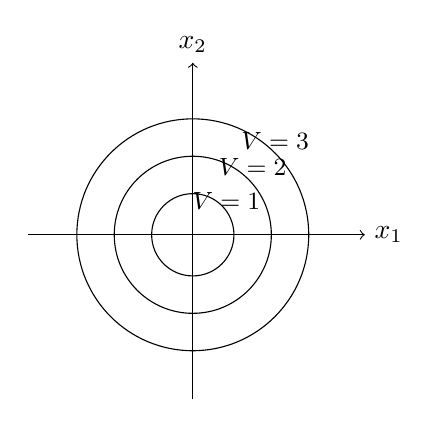
\begin{tikzpicture}[scale=0.95]
    \draw[->] (-2.2,0) -- (2.3,0) node[right] {$x_1$};
    \draw[->] (0,-2.2) -- (0,2.3) node[above] {$x_2$};
    \draw (0,0) circle (0.55);
    \draw (0,0) circle (1.05);
    \draw (0,0) circle (1.55);
    \node at (0.45,0.45) {\small \(V=1\)};
    \node at (0.8,0.9) {\small \(V=2\)};
    \node at (1.1,1.25) {\small \(V=3\)};
\end{tikzpicture}
\caption{Curve di livello di \(V(x_1,x_2)=x_1^2+x_2^2\): sono circonferenze concentriche.}
\end{figure}

\subsection*{Esempio 2: funzione negativa definita in un intorno dell'origine}
Consideriamo
\[
V(x_1,x_2)=\bigl(x_1^2+x_2^2\bigr)\bigl(x_1^2+x_2^2-2\bigr).
\]
Se ci restringiamo a una palla sufficientemente piccola, ad esempio \(\overline{B}_1\), allora:
\[
x_1^2+x_2^2 \ge 0,
\qquad
x_1^2+x_2^2-2 \le -1.
\]
Di conseguenza, per ogni \(x\neq 0\) con \(\|x\|\le 1\),
\[
V(x)<0.
\]
Inoltre \(V(0)=0\). Quindi \(V\) è negativa definita in \(\overline{B}_1\).

\begin{figure}[h!]
\centering
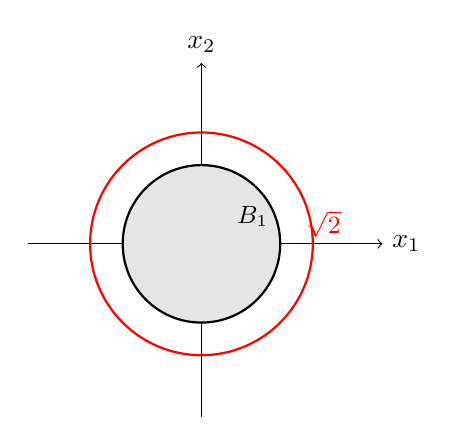
\begin{tikzpicture}[scale=1.0]
    \draw[->] (-2.2,0) -- (2.3,0) node[right] {$x_1$};
    \draw[->] (0,-2.2) -- (0,2.3) node[above] {$x_2$};
    \fill[gray!20] (0,0) circle (1.0);
    \draw[thick] (0,0) circle (1.0);
    \draw[red,thick] (0,0) circle (1.4142);
    \node at (0.65,0.35) {\small \(B_1\)};
    \node[red] at (1.55,0.25) {\small \(\sqrt{2}\)};
\end{tikzpicture}
\caption{In \(B_1\) il fattore \(x_1^2+x_2^2-2\) è sempre negativo, quindi \(V<0\) per ogni \(x\neq 0\).}
\end{figure}

\subsection*{Esempio 3: funzione negativa semidefinita}
Consideriamo
\[
V(x_1,x_2)=-x_2^2.
\]
Allora
\[
V(x_1,x_2)\le 0 \quad \forall (x_1,x_2),
\]
ma \(V=0\) per tutti i punti della forma \((x_1,0)\), non solo nell'origine.  
Quindi \(V\) è negativa semidefinita, ma non negativa definita.

\begin{figure}[h!]
\centering
\begin{tikzpicture}[scale=0.95]
    \draw[->] (-2.2,0) -- (2.3,0) node[right] {$x_1$};
    \draw[->] (0,-2.2) -- (0,2.3) node[above] {$x_2$};
    \draw[very thick] (-2,0) -- (2,0);
    \node[above right] at (0.15,0) {\small \(V=0\)};
\end{tikzpicture}
\caption{Per \(V(x_1,x_2)=-x_2^2\), la funzione si annulla su tutto l'asse \(x_1\).}
\end{figure}

\subsection*{Esempio 4: funzione indefinita}
Consideriamo
\[
V(x_1,x_2)=x_1^2-x_2^2.
\]
Se \(x_2=0\), allora \(V=x_1^2\ge 0\).  
Se \(x_1=0\), allora \(V=-x_2^2\le 0\).  
Quindi vicino all'origine la funzione assume sia valori positivi sia negativi: non è definita in segno.

\begin{figure}[h!]
\centering
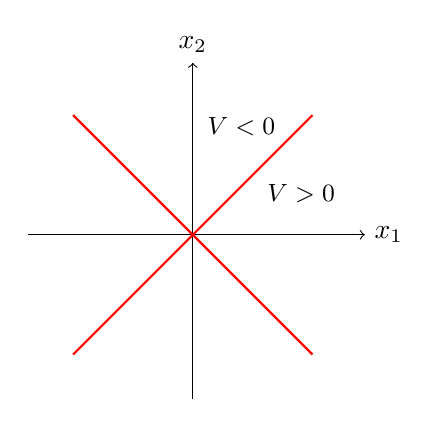
\begin{tikzpicture}[scale=0.95]
    \draw[->] (-2.2,0) -- (2.3,0) node[right] {$x_1$};
    \draw[->] (0,-2.2) -- (0,2.3) node[above] {$x_2$};

    \draw[red,thick] (-1.6,-1.6) -- (1.6,1.6);
    \draw[red,thick] (-1.6,1.6) -- (1.6,-1.6);

    \node at (1.45,0.55) {\small \(V>0\)};
    \node at (0.65,1.45) {\small \(V<0\)};
\end{tikzpicture}
\caption{Per \(V(x_1,x_2)=x_1^2-x_2^2\) il segno cambia a seconda della direzione.}
\end{figure}

\section{Forme quadratiche}

Un caso molto importante è quello in cui
\[
V(x)=x^\top Qx,
\]
dove \(Q\in\mathbb{R}^{n\times n}\).

\subsection{Riduzione alla parte simmetrica}
Ogni matrice \(Q\) si può decomporre come somma della sua parte simmetrica e della sua parte antisimmetrica:
\[
Q=Q_s+Q_a,
\]
dove
\[
Q_s=\frac{Q+Q^\top}{2},
\qquad
Q_a=\frac{Q-Q^\top}{2}.
\]
Vale
\[
Q_s^\top=Q_s,
\qquad
Q_a^\top=-Q_a.
\]

Ora osserviamo che, per ogni \(x\in\mathbb{R}^n\),
\[
x^\top Q_a x = 0.
\]
Infatti \(x^\top Q_a x\) è uno scalare, quindi coincide con la sua trasposta:
\[
x^\top Q_a x = (x^\top Q_a x)^\top = x^\top Q_a^\top x = x^\top(-Q_a)x = -x^\top Q_a x,
\]
da cui segue immediatamente
\[
x^\top Q_a x = 0.
\]

Pertanto
\[
V(x)=x^\top Qx=x^\top Q_s x.
\]
Quindi, nello studio del segno di una forma quadratica, conta solo la \textbf{parte simmetrica} della matrice.

\subsection{Caso simmetrico}
Se \(P=P^\top\), allora:
\[
V(x)=x^\top P x
\]
è positiva definita se e solo se tutti gli autovalori di \(P\) sono positivi.

Analogamente:
\begin{itemize}
    \item \(V\) è positiva semidefinita se gli autovalori di \(P\) sono non negativi;
    \item \(V\) è negativa definita se gli autovalori di \(P\) sono tutti negativi;
    \item \(V\) è indefinita se \(P\) ha autovalori di segno diverso.
\end{itemize}

\section{Idea del metodo diretto di Lyapunov}

Consideriamo un sistema non lineare autonomo tempo continuo
\[
\dot x = f(x),
\qquad
f(0)=0.
\]
Vogliamo capire se l'origine sia stabile, asintoticamente stabile oppure instabile, \emph{senza} risolvere esplicitamente il sistema.

L'idea di Lyapunov è costruire una funzione
\[
V:\mathbb{R}^n\to\mathbb{R}
\]
che giochi il ruolo di una specie di ``energia generalizzata''.

Se \(V\) è positiva definita e, lungo le traiettorie del sistema, il suo valore decresce, allora intuitivamente lo stato si muove verso l'origine.

\section{Derivata di \(V\) lungo le traiettorie}

\subsection{Caso continuo}
Se
\[
\dot x = f(x),
\]
allora la derivata temporale della funzione \(V(x(t))\) lungo una traiettoria \(x(t)\) è
\[
\frac{d}{dt}V(x(t))
=
\frac{\partial V}{\partial x}(x(t))\,\dot x(t)
=
\frac{\partial V}{\partial x}(x(t))\,f(x(t)).
\]
Questa quantità si indica con
\[
L_fV(x)=\nabla V(x)^\top f(x),
\]
e si chiama \textbf{derivata di Lie} di \(V\) rispetto al campo vettoriale \(f\), oppure più semplicemente \textbf{derivata di \(V\) lungo le traiettorie}.

\subsection{Caso discreto}
Se invece il sistema è tempo discreto
\[
x(k+1)=f(x(k)),
\]
si considera la variazione
\[
\Delta V(x(k)) = V(x(k+1))-V(x(k)).
\]

In entrambi i casi, il significato è lo stesso: misurare come cambia \(V\) mentre il sistema evolve.

\section{Interpretazione geometrica}

Se \(V\) è positiva definita, le sue curve di livello
\[
V(x)=c
\]
sono, intuitivamente, come ``linee di quota energetica'' attorno all'origine.

Se lungo le traiettorie vale
\[
L_fV(x)<0
\qquad\text{oppure}\qquad
\Delta V(x)<0,
\]
allora il sistema passa a livelli di energia sempre più bassi. Questo suggerisce che la traiettoria si sta avvicinando all'origine.

\begin{figure}[h!]
\centering
\begin{tikzpicture}[scale=1.0]
    % sinistra: superficie
    \begin{scope}
        \draw[->] (-1.8,0) -- (2.1,0) node[right] {$x_1$};
        \draw[->] (0,-1.6) -- (0,2.2) node[above] {$x_2$};
        \draw[->] (-1.0,-1.0) -- (-1.8,-1.8) node[left] {$V$};

        \draw (0,1.7) .. controls (0.8,1.6) and (1.2,1.0) .. (1.15,0.2);
        \draw (0,1.7) .. controls (-0.8,1.6) and (-1.2,1.0) .. (-1.15,0.2);
        \draw (-1.15,0.2) .. controls (-0.7,-0.15) and (0.7,-0.15) .. (1.15,0.2);
        \draw[dashed] (-0.75,0.35) .. controls (-0.45,0.15) and (0.45,0.15) .. (0.75,0.35);
        \node at (0.25,-0.45) {\small \(V=x_1^2+x_2^2\)};
    \end{scope}

    % destra: curve livello
    \begin{scope}[xshift=8cm]
        \draw[->] (-2.0,0) -- (2.2,0) node[right] {$x_1$};
        \draw[->] (0,-2.0) -- (0,2.2) node[above] {$x_2$};
        \draw (0,0) circle (0.45);
        \draw (0,0) circle (0.9);
        \draw (0,0) circle (1.35);
        \draw[->,thick] (1.3,0.2) -- (0.95,0.15);
        \draw[->,thick] (-1.15,-0.35) -- (-0.8,-0.25);
        \node at (0.55,0.45) {\small \(V=1\)};
        \node at (0.95,0.95) {\small \(V=2\)};
        \node at (1.35,1.35) {\small \(V=3\)};
    \end{scope}
\end{tikzpicture}
\caption{Interpretazione geometrica: se \(V\) decresce lungo le traiettorie, il sistema tende a muoversi verso curve di livello sempre più interne.}
\end{figure}

\section{Traslazione di un equilibrio non nullo}

Se il sistema ha un equilibrio in \(\bar x\neq 0\), non cambia nulla di concettuale: basta traslare le coordinate.

Poniamo
\[
z=x-\bar x.
\]
Allora l'equilibrio \(\bar x\) nel sistema originale diventa l'origine nel sistema traslato.

Perciò il metodo di Lyapunov si applica sempre, in sostanza, allo studio della stabilità dell'origine del sistema traslato.

\section{Insiemi di livello}

Per la dimostrazione del teorema diretto conviene introdurre alcuni insiemi standard.

Fissato un raggio \(\varepsilon>0\), indichiamo con
\[
B_\varepsilon=\{x\in\mathbb{R}^n:\|x\|<\varepsilon\},
\qquad
\partial B_\varepsilon=\{x\in\mathbb{R}^n:\|x\|=\varepsilon\}.
\]

Sia ora \(V\) una funzione positiva definita. Per un livello \(\rho>0\), definiamo:
\[
\Omega_\rho=\{x\in B_\varepsilon : V(x)\le \rho\},
\]
e la corrispondente curva/superficie di livello
\[
C_\rho=\partial\Omega_\rho
=
\{x\in B_\varepsilon : V(x)=\rho\}.
\]

\medskip

\noindent
L'idea è che, scegliendo \(\rho\) piccolo, l'insieme \(\Omega_\rho\) sia un intorno dell'origine contenuto in \(B_\varepsilon\).

\section{Teorema diretto di Lyapunov}

Consideriamo il sistema autonomo
\[
\dot x=f(x),
\qquad
f(0)=0,
\]
oppure, nel caso discreto,
\[
x(k+1)=f(x(k)),
\qquad
f(0)=0.
\]

Sia \(V\) una funzione positiva definita in un intorno dell'origine.

\subsection*{Enunciato}

\begin{enumerate}
    \item Se
    \[
    L_fV(x)\le 0
    \qquad
    \text{(oppure, nel discreto, } \Delta V(x)\le 0\text{)},
    \]
    allora l'origine è \textbf{stabile}.

    \item Se
    \[
    L_fV(x)<0
    \qquad
    \text{(oppure } \Delta V(x)<0\text{)}
    \]
    per ogni \(x\neq 0\), allora l'origine è \textbf{asintoticamente stabile}.

    \item Se
    \[
    L_fV(x)>0
    \qquad
    \text{(oppure } \Delta V(x)>0\text{)}
    \]
    per ogni \(x\neq 0\), allora l'origine è \textbf{instabile}.
\end{enumerate}

\medskip

\noindent
In questa lezione i passaggi di dimostrazione sono sviluppati soprattutto per il caso continuo. Il caso discreto è del tutto analogo, sostituendo l'integrale con somme finite e \(L_fV\) con \(\Delta V\).

\section{Lemma geometrico preliminare}

Prima della dimostrazione del teorema serve un fatto semplice ma fondamentale.

Sia \(V\) positiva definita e continua in \(\overline{B}_\varepsilon\). Allora:
\begin{enumerate}
    \item la funzione \(V\) ammette minimo su \(\partial B_\varepsilon\), perché \(\partial B_\varepsilon\) è compatto;
    \item tale minimo è strettamente positivo, perché su \(\partial B_\varepsilon\) non compare l'origine e \(V\) è positiva definita.
\end{enumerate}

Dunque, posto
\[
\alpha = \min_{x\in \partial B_\varepsilon} V(x),
\]
si ha
\[
\alpha>0.
\]

Ora scegliamo un numero \(\beta\) tale che
\[
0<\beta<\alpha.
\]
Allora il sottoinsieme di livello
\[
\Omega_\beta=\{x\in B_\varepsilon:V(x)\le \beta\}
\]
è contenuto strettamente dentro \(B_\varepsilon\), cioè
\[
\Omega_\beta \subset B_\varepsilon.
\]

Inoltre, essendo \(V(0)=0\) e \(V\) continua, esiste \(\delta>0\) tale che
\[
x\in B_\delta \quad \Longrightarrow \quad V(x)<\beta.
\]
Quindi
\[
B_\delta\subset \Omega_\beta.
\]

\medskip

\noindent
Questo lemma è esattamente il ponte che collega i livelli della funzione \(V\) con gli intorni metrici dell'origine.

\section{Dimostrazione del punto 1: stabilità}

Supponiamo che:
\[
V \text{ sia positiva definita},
\qquad
L_fV(x)\le 0.
\]

Vogliamo dimostrare che l'origine è stabile.

\subsection*{Passo 1: fissato un intorno finale, costruiamo un intorno iniziale}
Sia assegnato \(\varepsilon>0\).  
Per il lemma precedente, esiste \(\beta>0\) tale che
\[
B_\delta \subset \Omega_\beta \subset B_\varepsilon
\]
per un opportuno \(\delta>0\).

\subsection*{Passo 2: la traiettoria non può uscire da \(\Omega_\beta\)}
Prendiamo ora una traiettoria con condizione iniziale
\[
x(t_0)=x_0\in B_\delta.
\]
Allora, per costruzione,
\[
V(x_0)\le \beta.
\]

Poiché \(L_fV\le 0\), la funzione \(t\mapsto V(x(t))\) è non crescente. Dunque
\[
V(x(t))\le V(x_0)\le \beta
\qquad
\forall t\ge t_0.
\]
Quindi
\[
x(t)\in \Omega_\beta
\qquad
\forall t\ge t_0.
\]
Ma \(\Omega_\beta \subset B_\varepsilon\), perciò
\[
x(t)\in B_\varepsilon
\qquad
\forall t\ge t_0.
\]

\subsection*{Conclusione}
Abbiamo dimostrato che:
\[
\forall \varepsilon>0 \ \exists \delta>0
\quad \text{tale che} \quad
\|x_0\|<\delta
\Rightarrow
\|x(t)\|<\varepsilon \ \forall t\ge t_0.
\]
Questa è esattamente la definizione di stabilità.

\begin{figure}[h!]
\centering
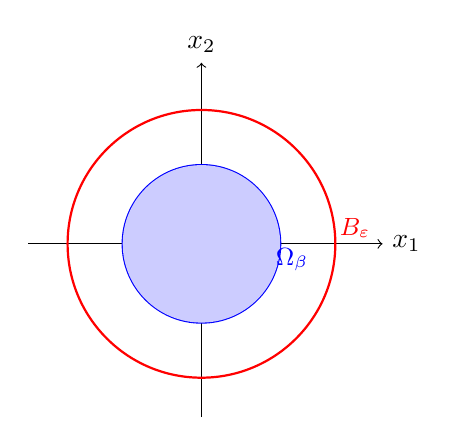
\begin{tikzpicture}[scale=1.0]
    \draw[->] (-2.2,0) -- (2.3,0) node[right] {$x_1$};
    \draw[->] (0,-2.2) -- (0,2.3) node[above] {$x_2$};

    \draw[red,thick] (0,0) circle (1.7);
    \draw[blue,thick] (0,0) circle (1.0);
    \fill[blue!20] (0,0) circle (1.0);

    \node[red] at (1.95,0.2) {\small \(B_\varepsilon\)};
    \node[blue] at (1.15,-0.2) {\small \(\Omega_\beta\)};
\end{tikzpicture}
\caption{Se \(V\) non cresce, una traiettoria che parte in \(\Omega_\beta\) non può uscirne.}
\end{figure}

\section{Dimostrazione del punto 2: stabilità asintotica}

Supponiamo ora che:
\[
V \text{ sia positiva definita},
\qquad
L_fV(x)<0 \quad \forall x\neq 0.
\]

Dal punto 1 sappiamo già che l'origine è stabile. Resta da dimostrare che è anche attrattiva, cioè
\[
x(t)\to 0 \qquad \text{per } t\to +\infty.
\]

\subsection*{Passo 1: \(V(x(t))\) è monotona e limitata inferiormente}
Per una traiettoria iniziale sufficientemente vicina all'origine, grazie alla stabilità essa resta in un insieme compatto \(\Omega_\beta\).  
La funzione \(V(x(t))\) è decrescente e soddisfa
\[
V(x(t))\ge 0.
\]
Dunque ammette limite:
\[
\lim_{t\to +\infty}V(x(t))=c
\qquad \text{con } c\ge 0.
\]

\subsection*{Passo 2: mostriamo che \(c=0\)}
Procediamo per assurdo. Supponiamo
\[
c>0.
\]
Scegliamo allora un valore intermedio
\[
0<d<c.
\]
Consideriamo l'anello compatto
\[
K=\Omega_\beta \setminus \operatorname{int}(\Omega_d).
\]
Su questo insieme vale:
\begin{itemize}
    \item \(K\) è compatto;
    \item \(0\notin K\);
    \item \(L_fV(x)<0\) per ogni \(x\in K\).
\end{itemize}
Per continuità, \(L_fV\) raggiunge massimo su \(K\); tale massimo è negativo, quindi esiste \(\gamma>0\) tale che
\[
L_fV(x)\le -\gamma
\qquad \forall x\in K.
\]

Poiché \(V(x(t))\to c>d\), per tempi sufficientemente grandi la traiettoria resta in \(K\). Quindi, per \(t\) abbastanza grande,
\[
\frac{d}{dt}V(x(t)) \le -\gamma.
\]
Integrando,
\[
V(x(t)) \le V(x(T))-\gamma(t-T),
\]
e facendo \(t\to+\infty\) si ottiene
\[
V(x(t))\to -\infty,
\]
che è impossibile perché \(V(x)\ge 0\).

Quindi l'assurdo mostra che
\[
c=0.
\]

\subsection*{Passo 3: da \(V(x(t))\to 0\) segue \(x(t)\to 0\)}
Fissiamo un qualunque \(\eta>0\).  
Poiché \(V\) è positiva definita, sulla sfera \(\partial B_\eta\) vale
\[
m_\eta := \min_{x\in \partial B_\eta}V(x) >0.
\]
Se per infiniti tempi fosse \(\|x(t)\|\ge \eta\), allora dovremmo avere
\[
V(x(t))\ge m_\eta >0,
\]
in contraddizione con \(V(x(t))\to 0\). Dunque
\[
x(t)\to 0.
\]

\subsection*{Conclusione}
L'origine è asintoticamente stabile.

\section{Dimostrazione del punto 3: instabilità}

Supponiamo infine che:
\[
V \text{ sia positiva definita},
\qquad
L_fV(x)>0 \quad \forall x\neq 0.
\]

Vogliamo dimostrare che l'origine è instabile.

\subsection*{Idea}
Se \(V\) cresce lungo le traiettorie, allora una traiettoria che parte molto vicina all'origine tende ad allontanarsi da livelli bassi di \(V\).  
Il ragionamento è speculare a quello usato per la stabilità.

\subsection*{Costruzione}
Sia fissato un piccolo \(\varepsilon>0\).  
Scegliamo un livello \(c>0\) tale che
\[
\Omega_c \subset B_\varepsilon.
\]
Prendiamo poi un livello \(a\) con
\[
0<a<c.
\]
La superficie
\[
C_a=\{x\in B_\varepsilon:V(x)=a\}
\]
può essere scelta arbitrariamente vicina all'origine scegliendo \(a\) piccolo.

Consideriamo l'anello compatto
\[
K=\Omega_c \setminus \operatorname{int}(\Omega_a).
\]
Su \(K\), la funzione \(L_fV\) è continua e strettamente positiva. Dunque esiste \(\gamma>0\) tale che
\[
L_fV(x)\ge \gamma
\qquad \forall x\in K.
\]

Se una traiettoria parte da un punto \(x_0\in C_a\) e rimanesse per sempre in \(\Omega_c\), allora finché resta in \(K\) si avrebbe
\[
\frac{d}{dt}V(x(t))\ge \gamma,
\]
da cui
\[
V(x(t))\ge a+\gamma(t-t_0).
\]
Quindi, in tempo finito, si arriverebbe a
\[
V(x(t))>c,
\]
il che contraddice l'ipotesi di permanenza in \(\Omega_c\).

Pertanto la traiettoria esce da \(\Omega_c\), e quindi anche da \(B_\varepsilon\).

\subsection*{Conclusione}
Esistono condizioni iniziali arbitrariamente vicine all'origine le cui traiettorie escono da un intorno prefissato dell'origine.  
Quindi l'origine è instabile.

\section{Osservazione importante}

Il teorema diretto di Lyapunov è estremamente potente perché consente di concludere la stabilità \emph{senza risolvere il sistema}.  
Il problema vero, nella pratica, è trovare una buona funzione \(V\).

In sintesi:
\begin{itemize}
    \item se troviamo \(V>0\) e \(L_fV\le 0\), otteniamo stabilità;
    \item se troviamo \(V>0\) e \(L_fV<0\), otteniamo stabilità asintotica;
    \item se troviamo \(V>0\) e \(L_fV>0\), otteniamo instabilità.
\end{itemize}

\section{Interpretazione energetica}

Il metodo di Lyapunov generalizza l'idea fisica di energia.

Se il sistema possiede una funzione energia \(E(x)\) che:
\begin{itemize}
    \item è minima nell'equilibrio;
    \item non aumenta lungo le traiettorie;
\end{itemize}
allora il sistema non può allontanarsi troppo dall'equilibrio.

Se addirittura tale energia diminuisce strettamente, allora il sistema dissipa energia e tende all'equilibrio.

\medskip

\noindent
Per questo motivo, nelle applicazioni meccaniche, spesso la funzione di Lyapunov si costruisce proprio a partire da energia cinetica e potenziale.

\section{Conclusioni della lezione}

In questa lezione abbiamo introdotto i concetti che stanno alla base della teoria diretta di Lyapunov:

\begin{enumerate}
    \item funzioni positive definite, semidefinite, negative definite e indefinite;
    \item forme quadratiche e loro riduzione alla sola parte simmetrica;
    \item derivata di una funzione lungo le traiettorie:
    \[
    L_fV(x)=\nabla V(x)^\top f(x)
    \quad \text{nel continuo},
    \qquad
    \Delta V(x)=V(x^+)-V(x)
    \quad \text{nel discreto};
    \]
    \item insiemi di livello e loro uso nella dimostrazione;
    \item teorema diretto di Lyapunov:
    \begin{itemize}
        \item \(L_fV\le 0 \Rightarrow\) stabilità,
        \item \(L_fV<0 \Rightarrow\) stabilità asintotica,
        \item \(L_fV>0 \Rightarrow\) instabilità.
    \end{itemize}
\end{enumerate}

Il cuore del metodo è questo: invece di cercare la soluzione del sistema, costruiamo una quantità scalare \(V\) che ci dica se il sistema tende ad avvicinarsi o ad allontanarsi dall'equilibrio.
